\documentclass[stu,12pt,floatsintext]{apa7}
\setlength\parindent{24pt}
% ============ Required Packages ============
\usepackage[english]{babel}  % Provides language-specific definitions
\usepackage[utf8x]{inputenc}  % Allows use of non-ASCII characters
\usepackage{amsmath,amssymb}  % Advanced math formatting
\usepackage{graphicx}  % Required for inserting images
\usepackage[colorinlistoftodos]{todonotes}  % Todo notes for draft versions
\setlength{\marginparwidth}{2cm}  % Set the margin width for todo notes
\usepackage{float}        % Enhanced figure positioning
\usepackage{booktabs}     % Professional table formatting
\usepackage{hyperref}     % Better link handling
\usepackage{csquotes}     % Improved quotation management

\usepackage{microtype}  % Improves typography
\usepackage{hyperref}   % Better link and reference handling
\usepackage{csquotes}   % Improved quotation handling

\usepackage{apacite} % APA citation style
\usepackage{natbib}  % Provides citation commands
\usepackage[table,xcdraw]{xcolor}
\bibliographystyle{apacite}  % APA citation style


% ============ Document Metadata ============
\title{Sentiment Analysis of Poverty Reddits}
\shorttitle{Sentiment Analysis}
\author{William W. Winters}
\authorsaffiliations{Anderson College of Business and Computing, Regis University}
\duedate{\today}
\course{MSDS 640: Ethics, Privacy, and Social Justice in Data Science}
\professor{Dr. Ghulam Mujtaba} 

% ============ Main Document ============
\begin{document}
\maketitle

% ============ Introduction Section ============
\section{Introduction}
\indent According to the \citet{uscensus2025}, there are 36.8 million people in the United States living at or below the poverty level.  Poverty and homelessness are problems that require a comprehensive solution to solve.  However, when viewed through a political lens, there are groups of people who view poor and homeless individuals as being in their predicament by making unwise decisions and have no one to blame but themselves for their situation.  This study will data mine posts from the poverty subReddit on the social media platform Reddit to determine what perceptions people have about poverty in the United States.  These posts will be examined using natural language processing (NLP) techniques to determine each posts sentiment using Valence Aware Dictionary and sEntiment Reasoner (VADER).  VADER not only provides a sentiment score of negative, neutral, and positive, it also indicates the intensity of the sentiment \citep{nltk2024}.
\section{Method}
\indent Using the Reddit API, a dataset consisting of approximately 1000 posts and their comments were download into a sqlite3 database.  The database was then queried to produce the dataframe used in this analysis.  After data cleaning and other preprocessing steps, the final dataset consisted of 8,110 rows and 13 features.  Text features related to the sentiment analysis being conducted were consolidated into a single feature and NLP text preparation techniques were applied.  Exploratory Data Analysis (EDA) was conducted on the dataframe to include the top ten word counts and other processes to assess the usefulness of the data.  See Figure 1 below.
\begin{figure}[H]
	\centering
	\caption{Top Ten Words from Poverty SubReddit}
	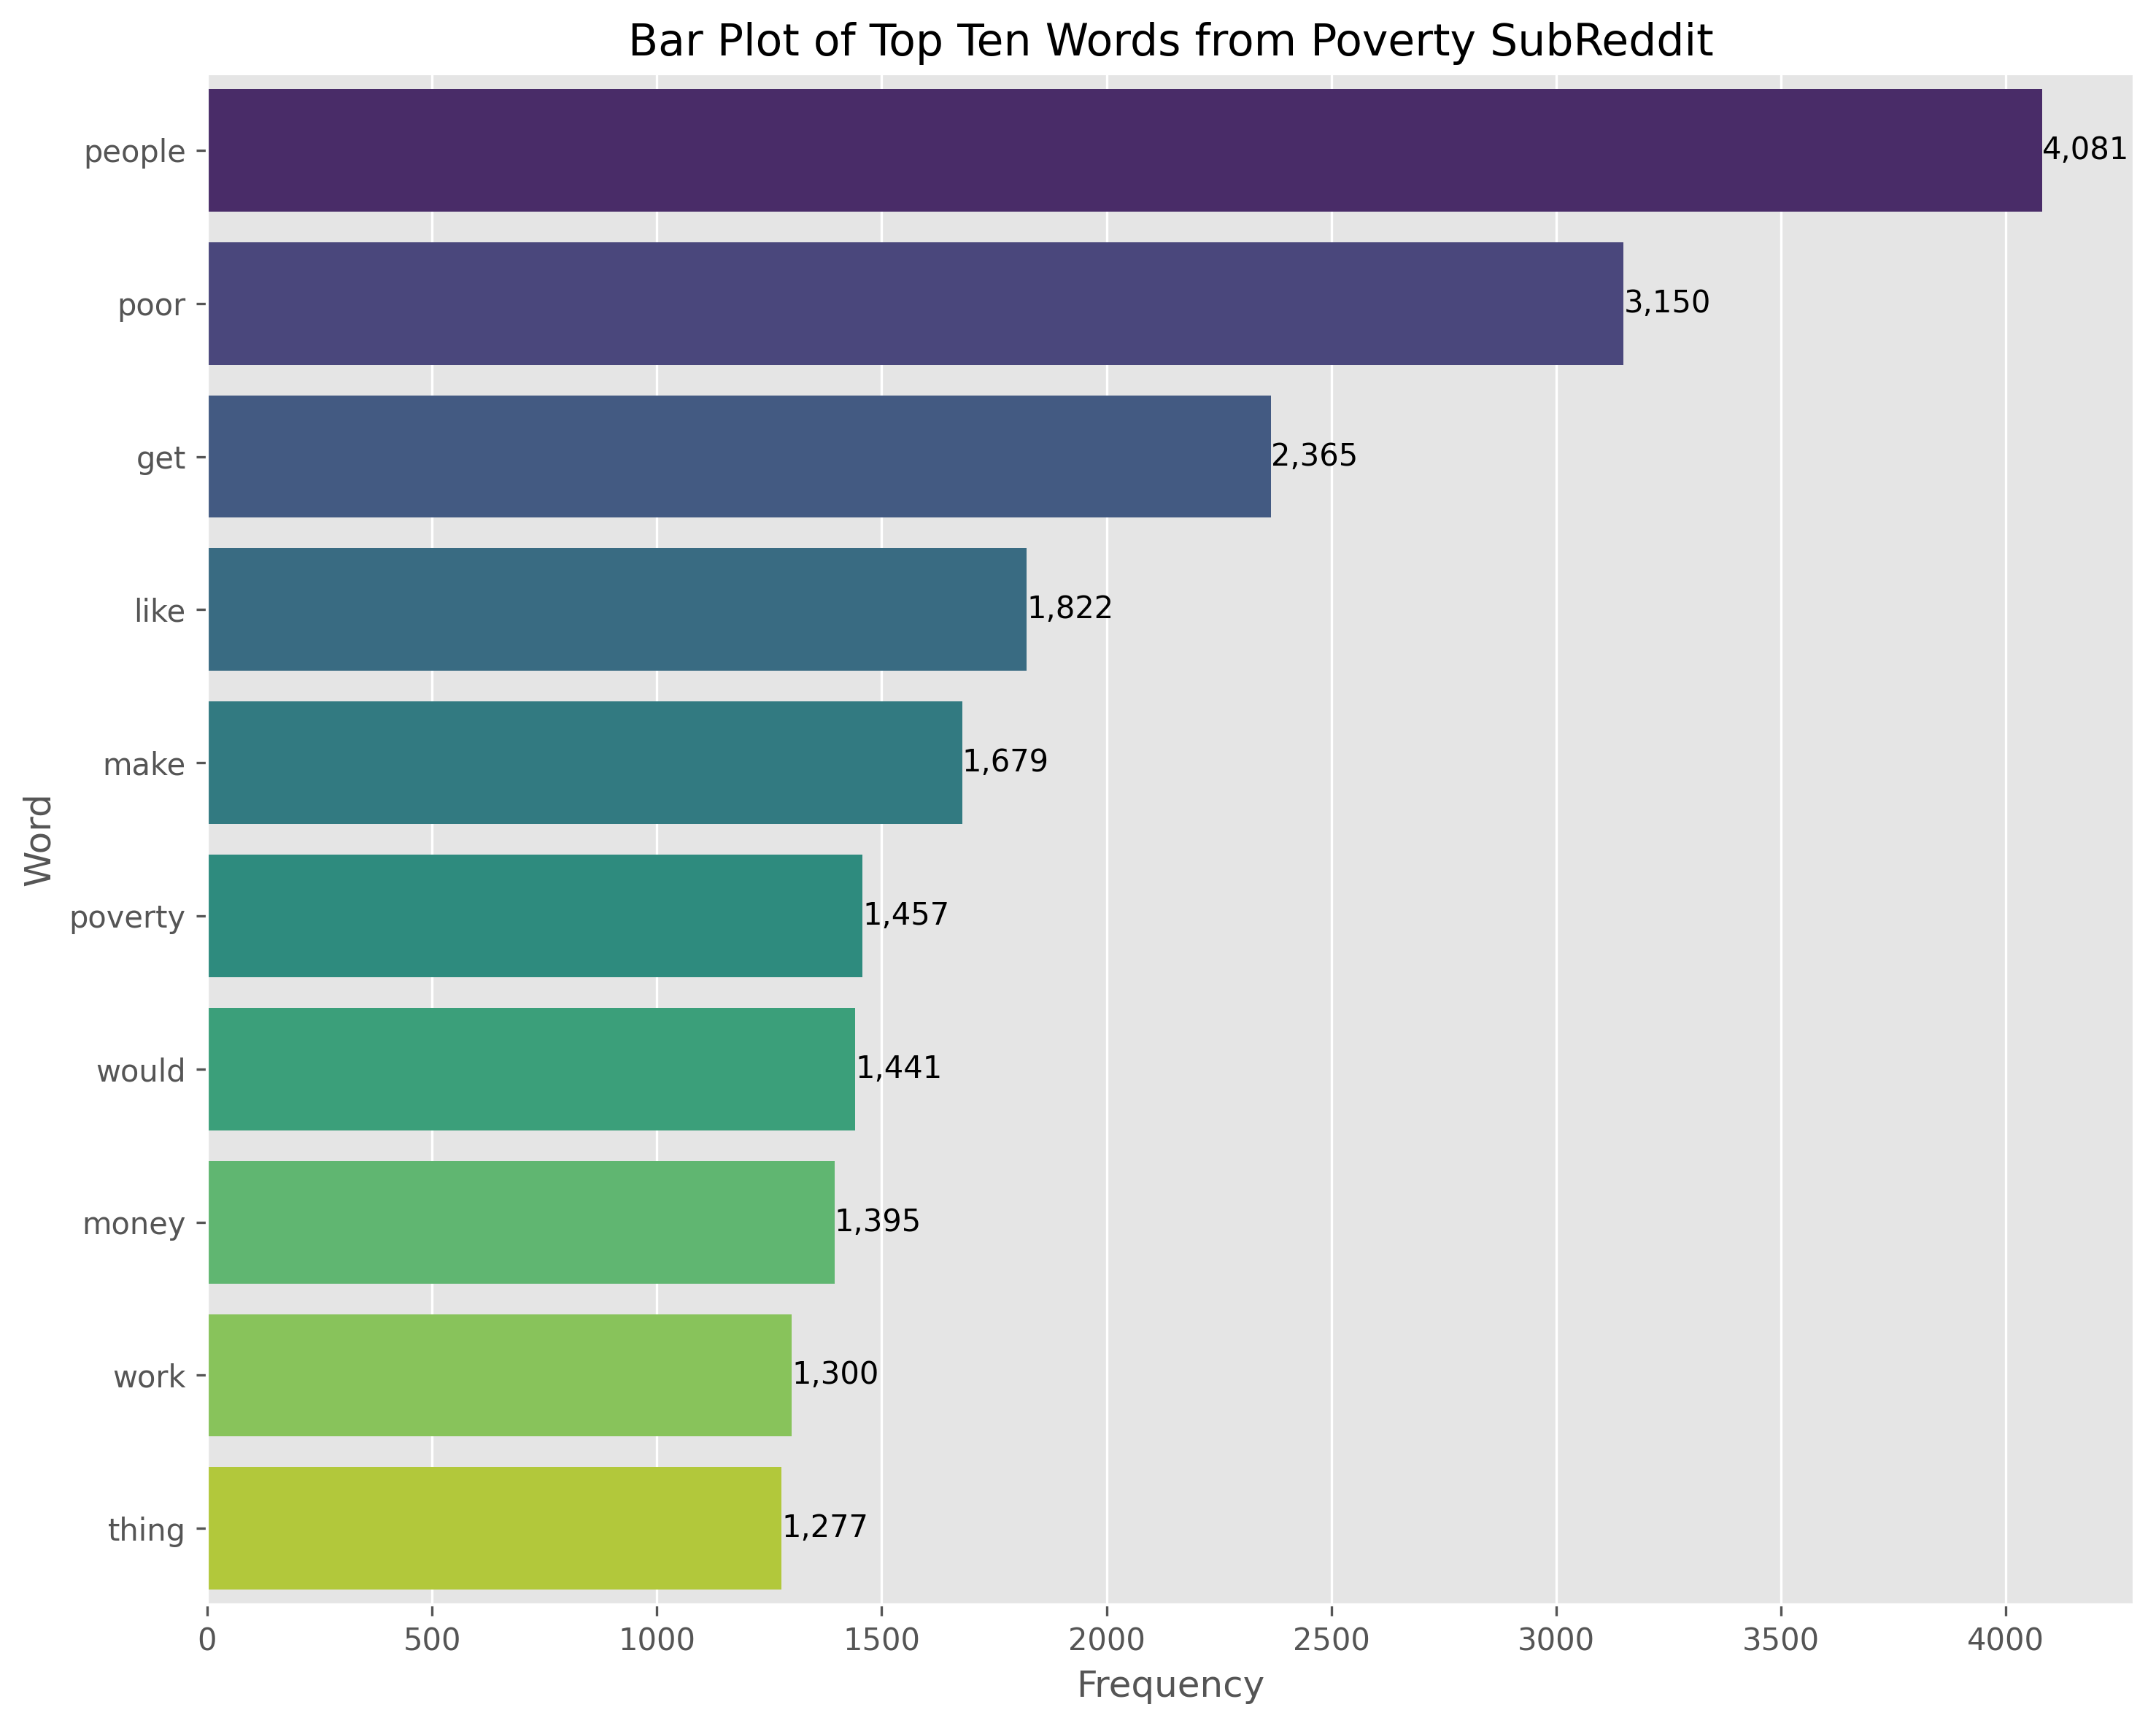
\includegraphics[width=0.75\linewidth]{figures/barplotWordCount.png}
	\label{fig:word_counts}
\end{figure}
\indent In some instances rows were dropped and in others columns were dropped or combined.  After EDA and some basic data cleaning, the text to be analyzed  was converted to lower case, numbers removed, punctuation removed, and extra spaces were handled.  All words except English stop words were lemmatized to prepare it for sentiment analysis. 

\indent VADER was applied to the processed text and a sentiment score for reach post was obtained.  The sentiment scores were limited to negative, neutral, and positive, although VADER can also provide the intensity of the sentiment.  The positive sentiment was the majority class, followed by negative and neutral. 
\begin{figure}[H]
	\centering
	\caption{Sentiment Analysis Counts}
	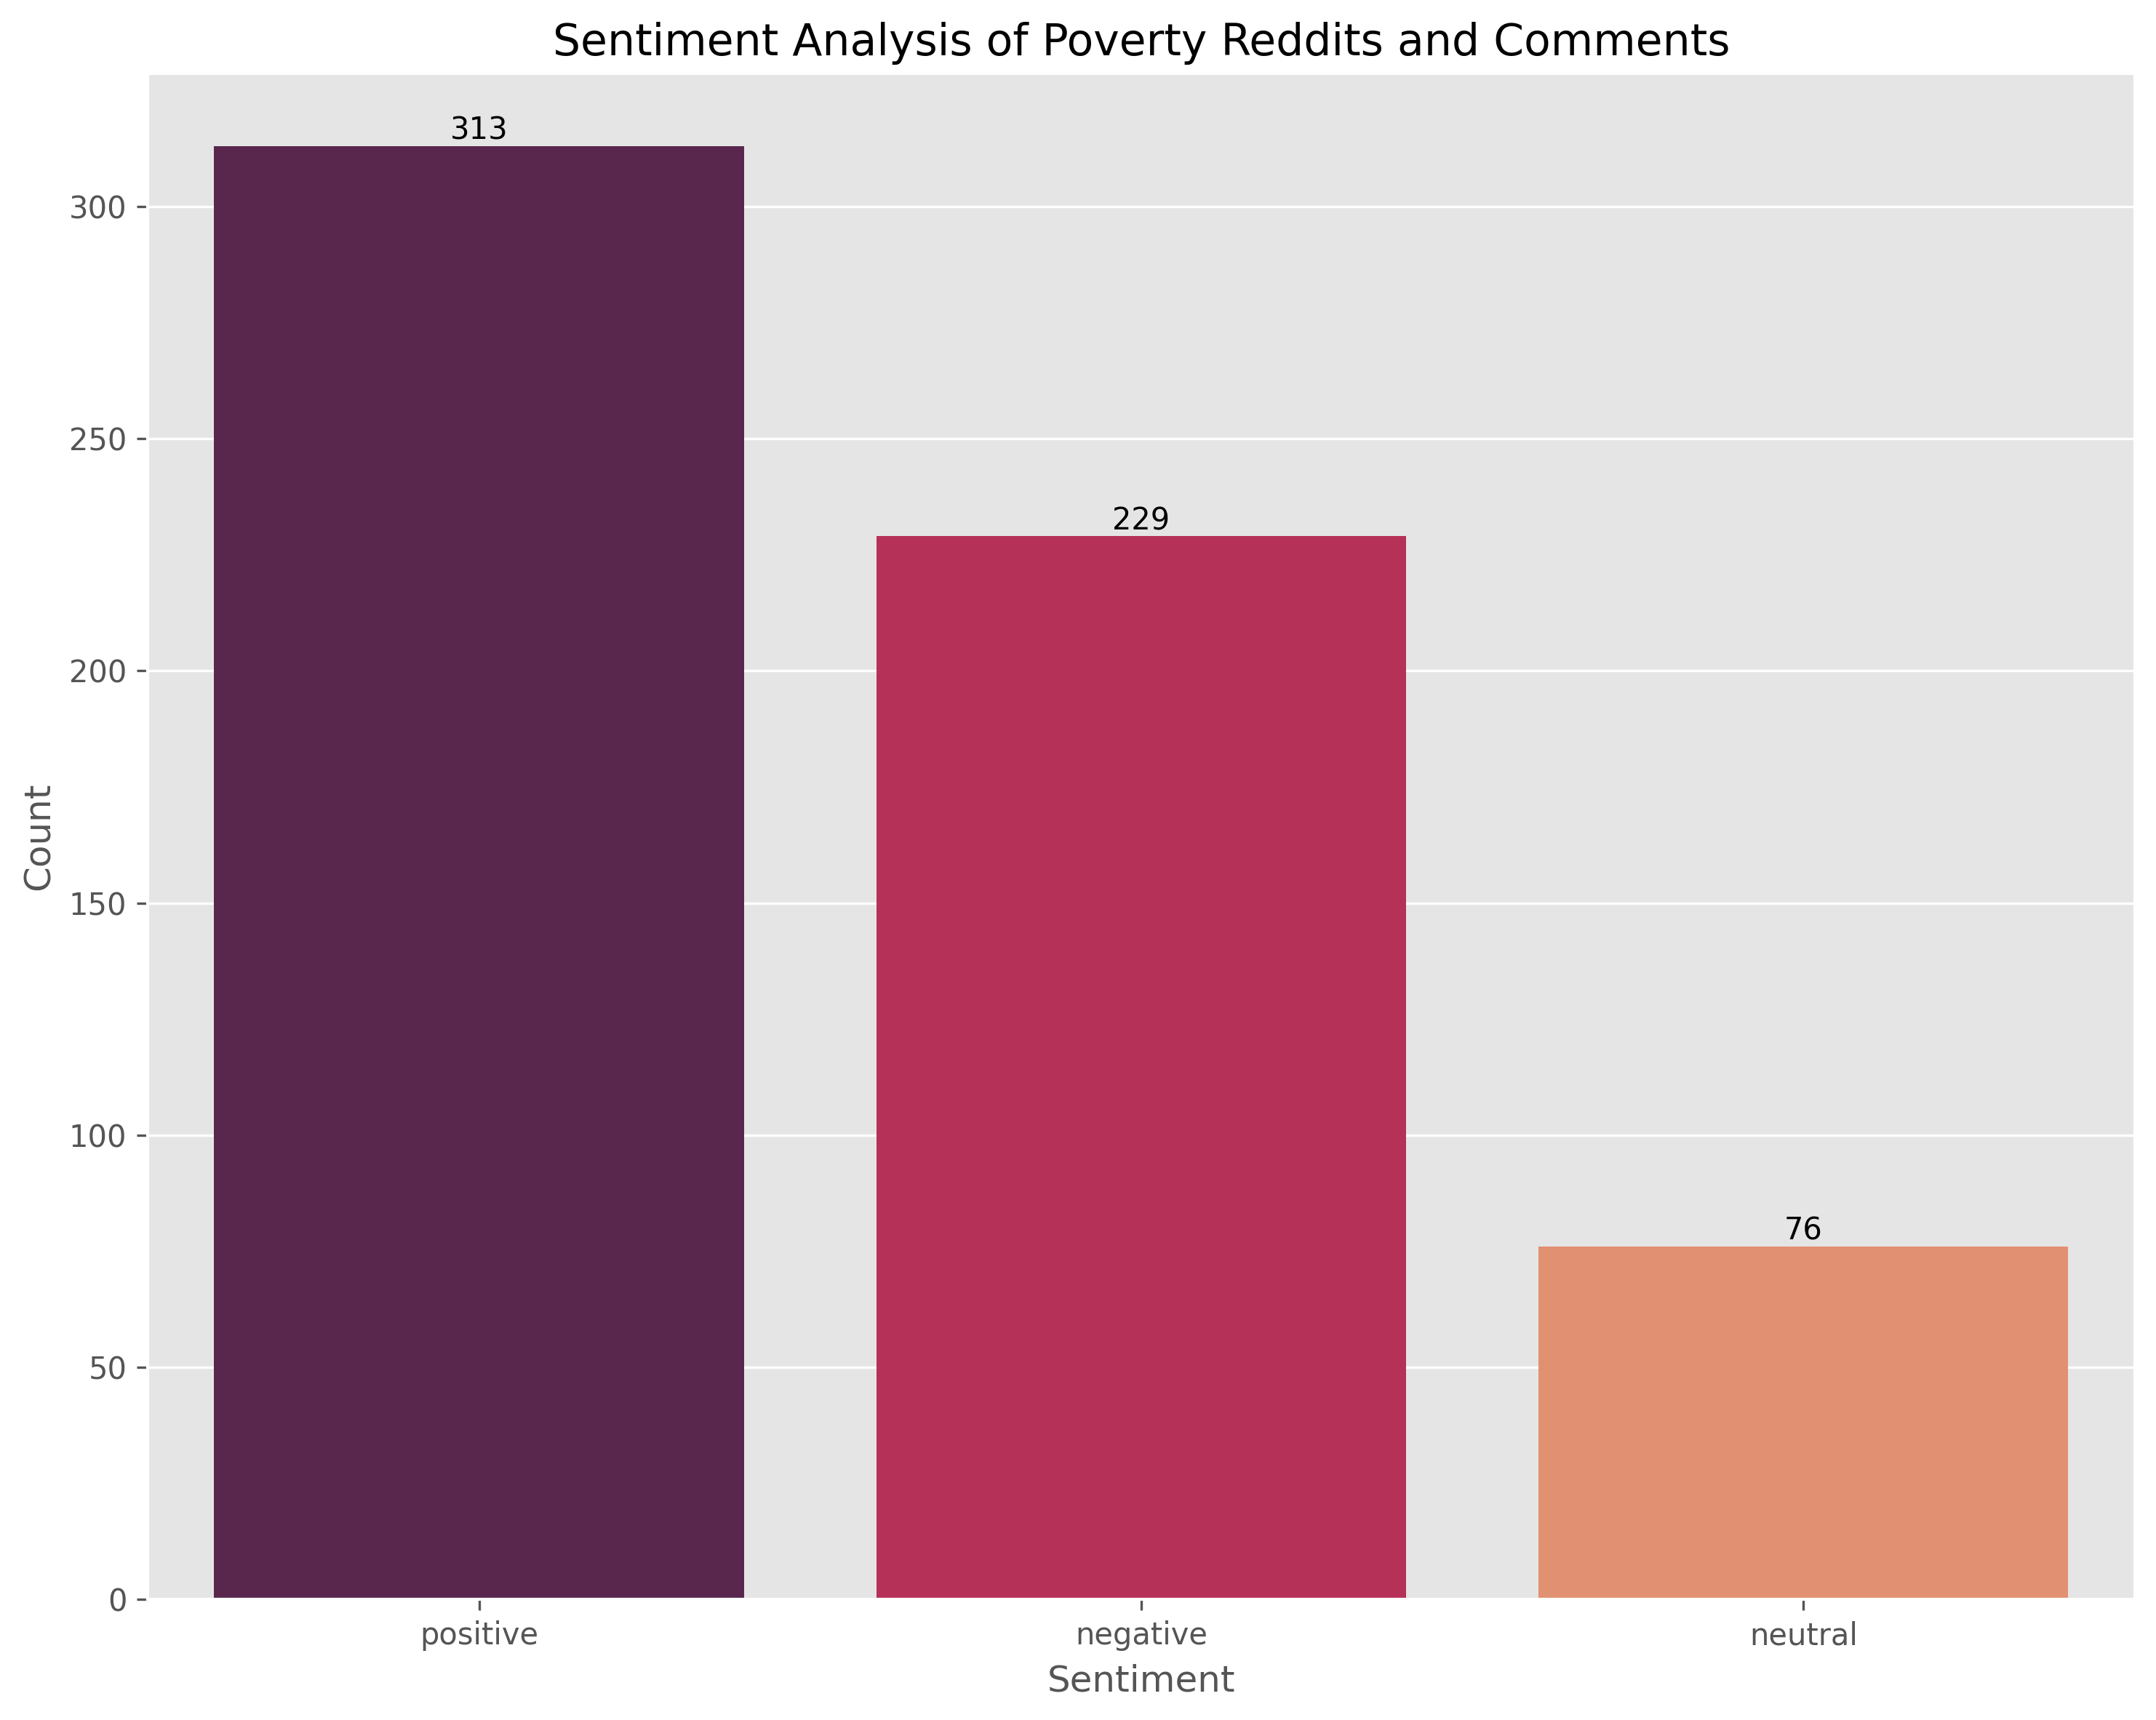
\includegraphics[width=0.75\linewidth]{figures/sentimentAnalysisSimple.png}
	\label{fig:sentiment_analysis}
\end{figure}
\section{Discussion}
\indent Many communities are affected by poverty and it is a complex issue with no easy answers.  Generally, it is believed that the effects of poverty could be reduced or minimized; yet, there is debate on whether it can be totally eliminated.  There are many causes of poverty in the U.S., but many agree that lower levels of education, lower levels of health, lack of access to affordable healthy food, and living in high-crime areas all contribute to individuals becoming impoverished.  While poverty is a complex issue with several causes, the only clear method of exiting it, is a quality education according to \citep{tackie2021}.

\indent One of the problems with poverty in the U.S. is people have different perceptions of the issue.  There is a large amount of stigma attached to being poor and maybe homeless and this makes it difficult to look at it as a social problem.  The extent to which the impoverished population is stigmatized reflects on the assumptions about the causes and possible policy solutions to the problem \citep{bowen2024}.  Which brings me back to the purpose of applying sentiment analysis to Reddit posts about poverty and that is does the Reddit community view it negatively or not.

\indent When data mining a social media platform, what obligations do researchers have to protect the privacy of the subjects engaging in activities in “public” internet spaces?  When using public internet spaces, is there an expectation of privacy?  This is a question that a growing number of researchers have been asking and has led to several professional organization issuing ethical guidelines governing the use of social media for research.  Although research practices vary from discipline to discipline and country to country, there are some common patterns that have emerged such as governments regulating internet-based research \citep{fiesler2024}.  The mind map below ties all of these concepts together.
\begin{figure}[H]
	\centering
	\caption{Poverty SubReddit Mind Map}
	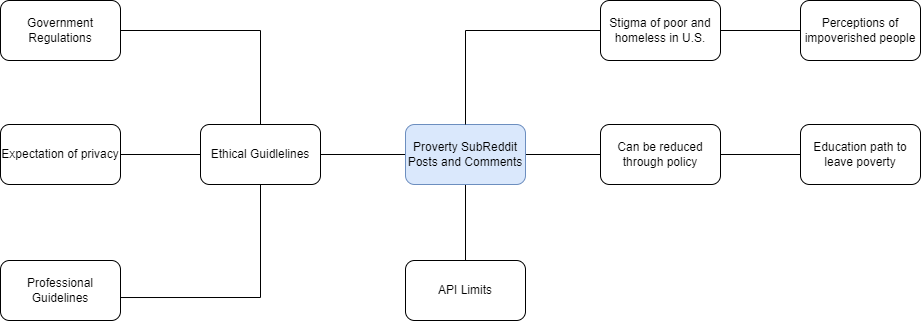
\includegraphics[width=0.75\linewidth]{figures/mindMapPoverty.png}
	\label{fig:mind_map}
\end{figure}
\section{Findings and Conclusions}
\indent The imbalance between positive, negative, and neutral sentiment classifications on the text data indicates poverty is a polarizing issue and many individuals in the Reddit community either post positively or negatively on the subject with not many being neutral.  In addition, the frequency of each sentiment was charted with its associated Reddit score range.  When a Reddit is posted, the community will either up-vote or down-vote it.  These votes are used to give the post a Reddit score.  The goal is to visualize any correlation between a Reddit score and the sentiments in the post.  No meaningful correlation was found; however, the Reddits that scored between 0 and 500, contained the largest numbers of comments.  Although the imbalance between the sentiment groups is concerning, the majority group.

\indent The literature review indicates poverty is a world-wide problem and there is no clear solution on how to solve it.  \citet{tackie2021} listed a quality education as a path out of poverty, but since it is a world-wide issue, education may not be the only answer.  Furthermore, ethical questions about the expectation of privacy was brought up and discussed by \citet{fiesler2024}.  According to his paper, this is an ethical dilemma with no clear answer at this time.    
% ============ References Section ============
\bibliography{references}

\end{document}
